\documentclass[10pt,letterpaper]{article}
\usepackage{geometry}
\geometry{letterpaper, portrait, margin=0.5in}
\usepackage[utf8]{inputenc}
\usepackage{amsmath}
\usepackage{amsfonts}
\usepackage{amssymb}
\usepackage{graphicx}
\usepackage{subcaption}
\usepackage{array}
\usepackage{hyperref}
\usepackage{adjustbox,lipsum}
\usepackage{gensymb}
\usepackage{listings}
\usepackage{color}
\usepackage{tikz}
\usepackage[makeroom]{cancel}
\setlength{\parindent}{0pt}
\renewcommand\refname{References}

\definecolor{mygreen}{rgb}{0,0.6,0}
\definecolor{mygray}{rgb}{0.5,0.5,0.5}
\definecolor{mymauve}{rgb}{0.58,0,0.82}

\lstset{ %
  backgroundcolor=\color{white},   % choose the background color; you must add \usepackage{color} or \usepackage{xcolor}
  %basicstyle=\tiny,        % the size of the fonts that are used for the code
  breakatwhitespace=false,         % sets if automatic breaks should only happen at whitespace
  breaklines=true,                 % sets automatic line breaking
  captionpos=b,                    % sets the caption-position to bottom
  commentstyle=\color{mygreen},    % comment style
  deletekeywords={...},            % if you want to delete keywords from the given language
  escapeinside={\%*}{*)},          % if you want to add LaTeX within your code
  extendedchars=true,              % lets you use non-ASCII characters; for 8-bits encodings only, does not work with UTF-8
  frame=single,	                   % adds a frame around the code
  keepspaces=true,                 % keeps spaces in text, useful for keeping indentation of code (possibly needs columns=flexible)
  keywordstyle=\color{blue},       % keyword style
  language=Python,                 % the language of the code
  otherkeywords={*,...},           % if you want to add more keywords to the set
  numbers=left,                    % where to put the line-numbers; possible values are (none, left, right)
  numbersep=5pt,                   % how far the line-numbers are from the code
  numberstyle=\tiny\color{mygray}, % the style that is used for the line-numbers
  rulecolor=\color{black},         % if not set, the frame-color may be changed on line-breaks within not-black text (e.g. comments (green here))
  showspaces=false,                % show spaces everywhere adding particular underscores; it overrides 'showstringspaces'
  showstringspaces=false,          % underline spaces within strings only
  showtabs=false,                  % show tabs within strings adding particular underscores
  stepnumber=2,                    % the step between two line-numbers. If it's 1, each line will be numbered
  stringstyle=\color{mymauve},     % string literal style
  tabsize=2,	                   % sets default tabsize to 2 spaces
  title=\lstname                   % show the filename of files included with \lstinputlisting; also try caption instead of title
}

\begin{document}
\title{\scshape\LARGE University of Waterloo \vfill \huge\bfseries PHYS 474 Assignment 2 \vfill}
\author{Robert Burnet \\ rcburnet@uwaterloo.ca \\ 20465122 }
\maketitle

\newpage
\begin{enumerate}
\item \begin{enumerate}
\item \begin{equation}\nonumber
\Phi (L) dL = n_* \left(\frac{L}{L_*}\right)^\alpha e^{-\frac{L}{L_*}} \frac{dL}{L_*}
\end{equation}
Number density of $L > 0.1 L_*$:
\begin{equation}\nonumber
\int_{0.1L_*}^{\infty} \Phi (L) dL = \int_{0.1L_*}^{\infty} n_* \left(\frac{L}{L_*}\right)^\alpha e^{-\frac{L}{L_*}} \frac{dL}{L_*}
\end{equation}
Numerically, in Python:
\begin{lstlisting}[language=Python]
import numpy as np
import matplotlib.pyplot as plt
from scipy import stats

def phi(L):
    n = 0.0037
    a = -0.96
    L_star = 10.0**11.0
    return n*(L/L_star)**a * np.e**(-L/L_star) / L_star

x = np.linspace(10**10, 10**13, 1000000)

result = np.trapz(phi(x), x)

print "space density:", result
\end{lstlisting}
Which gives $\int_{0.1L_*}^{\infty} \Phi (L) dL \approx \textbf{0.00646  Mpc$^{-3}$}$\\

This means that in every volume of 1 Mpc$^3$, we'd see 0.00646 galaxies within, or we'd see approximately 1 galaxy in a volume of 154.8 Mpc$^3$, which corresponds to a galaxy separation of:
\begin{equation}\nonumber
\begin{split}
V & =  \frac{4}{3} \pi R^3 \\
\Rightarrow R & = \sqrt[3]{\frac{3V}{4\pi}} \\
& = \textbf{3.33 Mpc$^3$}
\end{split}
\end{equation}

To get the number of galaxies in the universe, simply multiply the space density of galaxies by the volume of the universe:
\begin{equation}\nonumber
\begin{split}
\# & = 0.00646\text{Mpc}^{-3} (V_{universe})\\
 & = 0.00646 \left(\frac{4}{3} \pi R_H^3\right)\\
 & = \textbf{7.43$\times$10$^{10}$ galaxies}
\end{split}
\end{equation}

\item Luminosity density of $L > 0$, $\rho_{L>0}$:
\begin{equation}\nonumber
\int_{0}^{\infty} \Phi (L) L dL = \int_{0}^{\infty} n_* \left(\frac{L}{L_*}\right)^{\alpha+1} e^{-\frac{L}{L_*}} dL
\end{equation}
Luminosity density of $L > 0.1 L_*$, $\rho_{L>0.1L_*}$:
\begin{equation}\nonumber
\int_{0.1L_*}^{\infty} \Phi (L) L dL = \int_{0.1L_*}^{\infty} n_* \left(\frac{L}{L_*}\right)^{\alpha+1} e^{-\frac{L}{L_*}} dL
\end{equation}
Numerically, in Python:
\begin{lstlisting}[language=Python]
import numpy as np
import matplotlib.pyplot as plt
from scipy import stats

def phiL(L):
    n = 0.0037
    a = -0.96
    L_star = 10.0**11.0
    return n*(L/L_star)**(a+1) * np.e**(-L/L_star)

x_0 = np.linspace(0, 10**13, 1000000)
x_10 = np.linspace(10**10, 10**13, 1000000)

result_0 = np.trapz(phiL(x_0), x_0)
result_10 = np.trapz(phiL(x_10), x_10)
    
print "L > 0 luminosity density:", result_0
print "L > 0.1 L_star luminosity density:", result_10
\end{lstlisting}
Which gives $\int_{0}^{\infty} \Phi (L) L dL \approx \textbf{3.62$\times$10$^{8}$ L$_\odot$/Mpc$^3$}$\\

and $\int_{0.1 L_*}^{\infty} \Phi (L) L dL \approx \textbf{3.31$\times$10$^{8}$ L$_\odot$/Mpc$^3$}$\\

and $\frac{\rho_{L>0.1L_*}}{\rho_{L>0}} = \textbf{0.91}$\\

Therefore, they make up about 91\% of the luminosity density of the universe.

\item \begin{equation}\nonumber
\begin{split}
\frac{0.3 \rho_{crit}}{\rho_{L>0}} & = \frac{0.3\left(\frac{3H_0^2}{8 \pi G}\right)}{3.62\times10^{8}}\\
 & = 2.24 \times 10^{32} kg/L_\odot\\
 & = \textbf{112.7 M$_\odot$/L$_\odot$}
\end{split}
\end{equation}
Where $H_0$ = $(70\text{km/s/Mpc})(\frac{3.2408\times10^{-20}\text{Mpc}}{1\text{km}})$ = $2.2686\times10^{-18}\text{s}^{-1}$ \\
and $G$ = $(6.674\times10^{-11}\text{m}^3\text{/kg/s}^2)(\frac{3.2408\times10^{-20}\text{Mpc}}{1000\text{m}})^3$ = $2.272\times10^{-78}\text{Mpc}^3\text{/kg/s}^2$\\

\item The largest value for $M/L_*$ I could obtain was 2.31 with age of 13.7 Gyrs and metallicity of -1.999. My calculated value was $\approx$ 49 times larger than the value I obtained from the model.\\

\item 
\begin{equation}\nonumber
\begin{split}
M \propto L \Rightarrow M = 112.7 \frac{M_\odot}{L_\odot} L\\
M_{universe} = M_{DM, universe}\\
\end{split}
\end{equation}
\begin{center}
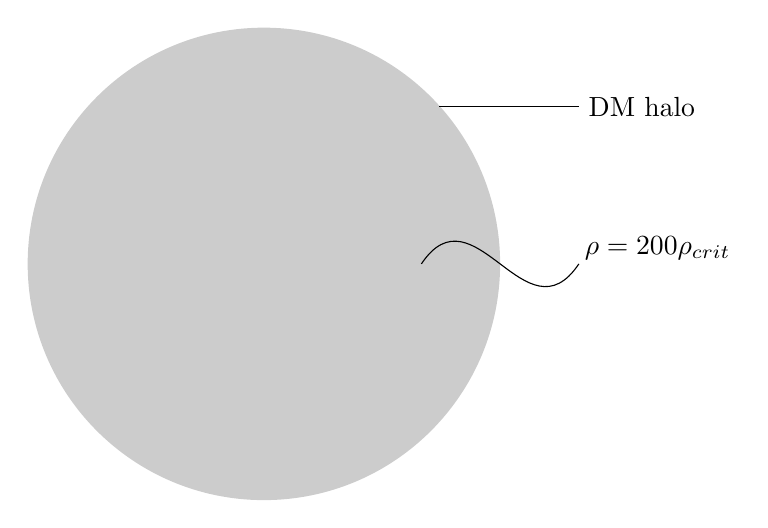
\begin{tikzpicture}
\fill[gray!40!white] (2,2) circle (3cm);
\draw (4.23,4) -- (6,4); 
\node at (6.8,4) {DM halo};
\draw (4,2) .. controls (4.67,3) and (5.33,1) .. (6,2); 
\node at (7,2.2) {$\rho = 200\rho_{crit}$};
\end{tikzpicture}
\end{center}

\newpage

\begin{equation}\nonumber
\begin{split}
@ L_* \Rightarrow M_* & = 112.7 \frac{M_\odot}{\cancel{L_\odot}} 10^{11}\cancel{L_\odot}\\
 & = 1.127 \times 10^{13} M_\odot
\end{split}
\end{equation}

\begin{equation}\nonumber
\begin{split}
\rho & = 200\rho_{crit}\\
 & = 200(\left(\frac{3 H_0^2}{8 \pi G}\right))\\
 & = 5.4083 \times 10^{43} \text{kg/Mpc}^3\\
 & = 2.7192 \times 10^{13} M_\odot/\text{Mpc}^3
\end{split}
\end{equation}

\begin{equation}\nonumber
\begin{split}
\rho & = \frac{M}{V}\\
2.71920\times10^{13}M_\odot/\text{Mpc}^3 & = \frac{1.127\times10^{13}M_\odot}{\frac{4}{3} \pi R^3}\\
R & = \sqrt[3]{\frac{1.127\times10^{13}}{2.7192 \times10^{13}}\left(\frac{3}{4\pi}\right)}\\
 & = \textbf{0.463 Mpc}\\
\end{split}
\end{equation}

\item 
\begin{equation}\nonumber
M_{K,MW} = -24.0\\
\end{equation}
\begin{equation}\nonumber
M_{V, \odot} - M_{K, \odot} = V_\odot - K_\odot\\
\end{equation}
\begin{equation}\nonumber
4.83 - M_{K, \odot} = 1.52 \text{ (From Table 1.4)}\\
\end{equation}
Therefore, 
\begin{equation}\nonumber
M_{K, \odot} = 3.31\\
\end{equation}

\begin{equation}\nonumber
M_{K, MW} = M_{K, \odot} - 2.5 log \left(\frac{L}{L_\odot}\right)\\
\end{equation}
\begin{equation}\nonumber
\Rightarrow \frac{L_{MW}}{L_\odot} = 10^{0.4(3.31 - M_{K, MW})}\\
\end{equation}

Therefore, 
\begin{equation}\nonumber
\begin{split}
L_{MW} & = \textbf{8.39$\times$10$^{10} L_\odot$}\\
 & = \textbf{0.839 $L_*$}\\
\end{split}
\end{equation}

as in e), \begin{equation}\nonumber
\begin{split}
R & = \sqrt[3]{\frac{112.7\times0.839\times10^{11}}{2.7192 \times10^{13}}\left(\frac{3}{4\pi}\right)}\\
 & = \textbf{0.436 Mpc}\\
\end{split}
\end{equation}

\item
\begin{equation}\nonumber
M_{K, M31} = -24.5\\
\end{equation}
\begin{equation}\nonumber
\frac{L_{M31}}{L_\odot} = 10^{0.4(3.31 - M_{K, M31})}\\
\end{equation}
\begin{equation}\nonumber
\begin{split}
L_{M31} & = \textbf{1.33 $\times$ 10$^{11} L_\odot$}\\
 & = \textbf{1.33 $L_*$}\\
\end{split}
\end{equation}

as in e), \begin{equation}\nonumber
\begin{split}
R & = \sqrt[3]{\frac{112.7\times1.33\times10^{11}}{2.7192 \times10^{13}}\left(\frac{3}{4\pi}\right)}\\
 & = \textbf{0.509 Mpc}\\
\end{split}
\end{equation}


\end{enumerate}

\item 
\begin{enumerate}

\item

\begin{lstlisting}[language=Python]
log_cz = np.array([3.958, 4.066, 4.223, 3.992, 4.137, 3.897, 3.891, 4.481, 3.774, 4.240, 3.736, 4.326])
m = np.array([16.4090, 17.3488, 17.8124, 16.3683, 17.2548, 16.2426, 16.2164, 19.0955, 15.4026, 17.7777, 15.4329, 18.4524])

# Linear regression to find best fit line:
slope, intercept, r_value, p_value, std_err = stats.linregress(log_cz, m)

std_dev = np.std(m)

print "std_err with fitted slope:", std_err
print "fitted slope:", slope
print "intercept with fitted slope:", intercept

# Do it for fixed slope of 5.0:
slope_fixed = 5.0
intercepts_fixed = m - slope_fixed*log_cz
intercept_fixed = np.mean(intercepts_fixed)

std_intercepts = np.std(intercepts_fixed)

print "intercept with fixed slope:", intercept_fixed

print "standard deviation of magnitudes:", std_dev
print "standard deviation of intercepts:", std_intercepts

lobf_fit = slope*log_cz + intercept
lobf_fixed = slope_fixed*log_cz + intercept_fixed

points = plt.scatter(log_cz, m, s = 2, color='b')
line1 = plt.plot(log_cz, lobf_fit)
line2 = plt.plot(log_cz, lobf_fixed)
plt.setp(line1, color='r', linewidth=0.3)
plt.setp(line2, color='g', linewidth=0.3)
plt.title('$m_{max}$ vs log$_{10}$($\\frac{cz}{[km/s]}$)')
plt.ylabel('$m_{max}$')
plt.xlabel('log$_{10}$($\\frac{cz}{[km/s]}$)')
plt.savefig('a02q2ae.png')
\end{lstlisting}

\begin{figure}[h!]
\centering
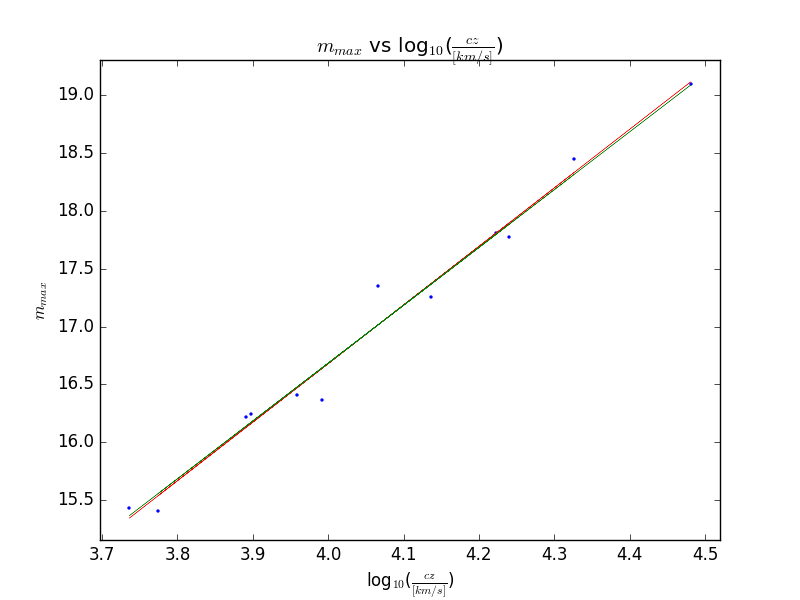
\includegraphics[scale=0.8]{a02q2ae.png}
\end{figure}

\newpage

\item \begin{equation}\nonumber
M = m - 5 log \left(\frac{d}{10}\right)
\end{equation}
Where M is constant
\begin{equation}\nonumber
cz = H_0 d \times \frac{1 \text{Mpc}}{10^6 \text{pc}} \Rightarrow d = \frac{cz}{H_0}\times 10^6
\end{equation}
\begin{equation}\nonumber
\Rightarrow M_{max} = m_{max} - 5 log \left(\frac{cz}{H_0}10^5\right)
\end{equation}
Therefore,
\begin{equation}\nonumber
m_{max} = 5 log(cz) - 5 log \left(\frac{H_0}{10^5}\right) + M_{max}
\end{equation}
This is a line of $m_{max}$ vs $log(cz)$ with a slope of 5.0 and intercept of $M_{max} - 5log\left(\frac{H_0}{10^5}\right)$\\

\item as above, the intercept is $M_{max} - 5log\left(\frac{H_0}{10^5}\right)$\\
\begin{equation}\nonumber
\Rightarrow m_0 = M_{max} - 5 log \left(\frac{h}{10^3}\right)
\end{equation}
Where $h = \frac{H_0}{100 \text{km/s/Mpc}}$\\

\item
\begin{enumerate}
\item redshift and $m_{max}$ measurements may have uncertainties which result in discrepancy between expected and actual values that aren't accounted for here.\\
\item $m_{max}$ is flux dependent, which depends on intensity of light on CCD camera. Light from different parts of the sky go through different amounts of dust and may be absorbed more or less than other light sources.\\
\item the second reason is probably more significant as the data is given to us to 4 and 6 significant digits, which an uncertainty of $\pm$ 0.0005 for $log(cz)$ and $\pm$ 0.00005 for $m_{max}$ wouldn't account for the amount of discrepancy seen, assuming all the digits reported in the table are certain.\\
\end{enumerate}

\item from output of code above in a):\\

standard error = 0.2188 (statistical uncertainty of slope)\\
slope = 5.065 $\approx$ 5.1\\
intercept = -3.580\\

Our expectations are a slope of 5.0, I get a slope of 5.1 which, with a standard error of 0.2188, is consistent with our expectations.\\

With fixed slope of 5.0, I get an intercept of -3.316, with standard deviation (uncertainty of intercept) of 0.151.\\

The standard deviation in magnitudes of the points is 1.114.\\

See plot above in a) for plotted lines of best fit.\\

\item \begin{equation}\nonumber
m_0 = M_{max} - 5 log \left(\frac{h}{10^3}\right)
\end{equation}
\begin{equation}\nonumber
\begin{split}
m_{max} - M_{max} & = 32.0 \text{ (for NGC 4639)}\\
12.61 - M_{max} & = 32.0\\
\Rightarrow M_{max} & = -19.39\\
\end{split}
\end{equation}
Therefore, 
\begin{equation}\nonumber
m_0 = -19.39 - 5 log\left(\frac{h}{10^3}\right)
\end{equation}

I found that $m_0$ = -3.580 for fitted slope, and -3.316 for fixed slope.\\

Therefore, $h_1$ $\approx$ 0.69 for the fitted slope (slope $\approx$ 5.1) and $h_2$ $\approx$ 0.61 for the fixed slope (slope = 5.0).\\

\begin{equation}\nonumber
h_{ave} = \frac{h_1 + h_2}{2} \approx \textbf{0.65}
\end{equation}

\item \begin{equation}\nonumber
\begin{split}
h & = 10^{\frac{- m_0+19.39}{5}+3}\\
dh & = \pm |\frac{\partial h}{\partial m_0}| |d m_0|\\
 & = \pm | -0.0609882 \times 10^{\frac{-m_0}{5}} | | d m_0 |\\
\end{split}
\end{equation}
Where $m_0 = -3.58$ or $= -3.316$ and $|d m_0| = 0.151$\\

Therefore,\\
\begin{equation}\nonumber
\begin{split}
dh_1 & = \pm 0.048 \text{ (for $m_0 = -3.58$)}\\
dh_2 & = \pm 0.042 \text{ (for $m_0 = -3.316$)}\\
\end{split}
\end{equation}
Therefore,\\
\begin{equation}\nonumber
\begin{split}
dh_{ave} & = \pm \sqrt{\left(\frac{\partial h_{ave}}{\partial h_1} dh_1\right)^2 + \left(\frac{\partial h_{ave}}{\partial h_2} dh_2 \right)^2}\\
 & = \pm \sqrt{\frac{1}{4}\left(dh_1^2 + dh_2^2\right)}\\
 & = \pm \frac{1}{2} \sqrt{dh_1^2 + dh_2^2}\\
 & = \pm \textbf{0.032}\\
\end{split}
\end{equation}
\end{enumerate}
\end{enumerate}

\end{document}